\sffamily
Here you can see how to include an image in your document.

Here is the command to refer to another element (section, figure, table, ...) in the document: \emph{As discussed in Section~\ref{sect:overview} and as shown in Figure~\ref{fig:metamodel}, ...}. Here is how to introduce a bibliographic citation~\cite{DAM}. Bibliographic references should be included in a \texttt{.bib} file. 

Table generation is a bit complicated in Latex. You will soon become proficient, but to start you can rely on tools or external services. See for instance this \href{https://www.tablesgenerator.com}{https://www.tablesgenerator.com}. \\

\subsection{\sffamily Product Perspective}
\begin{figure}
	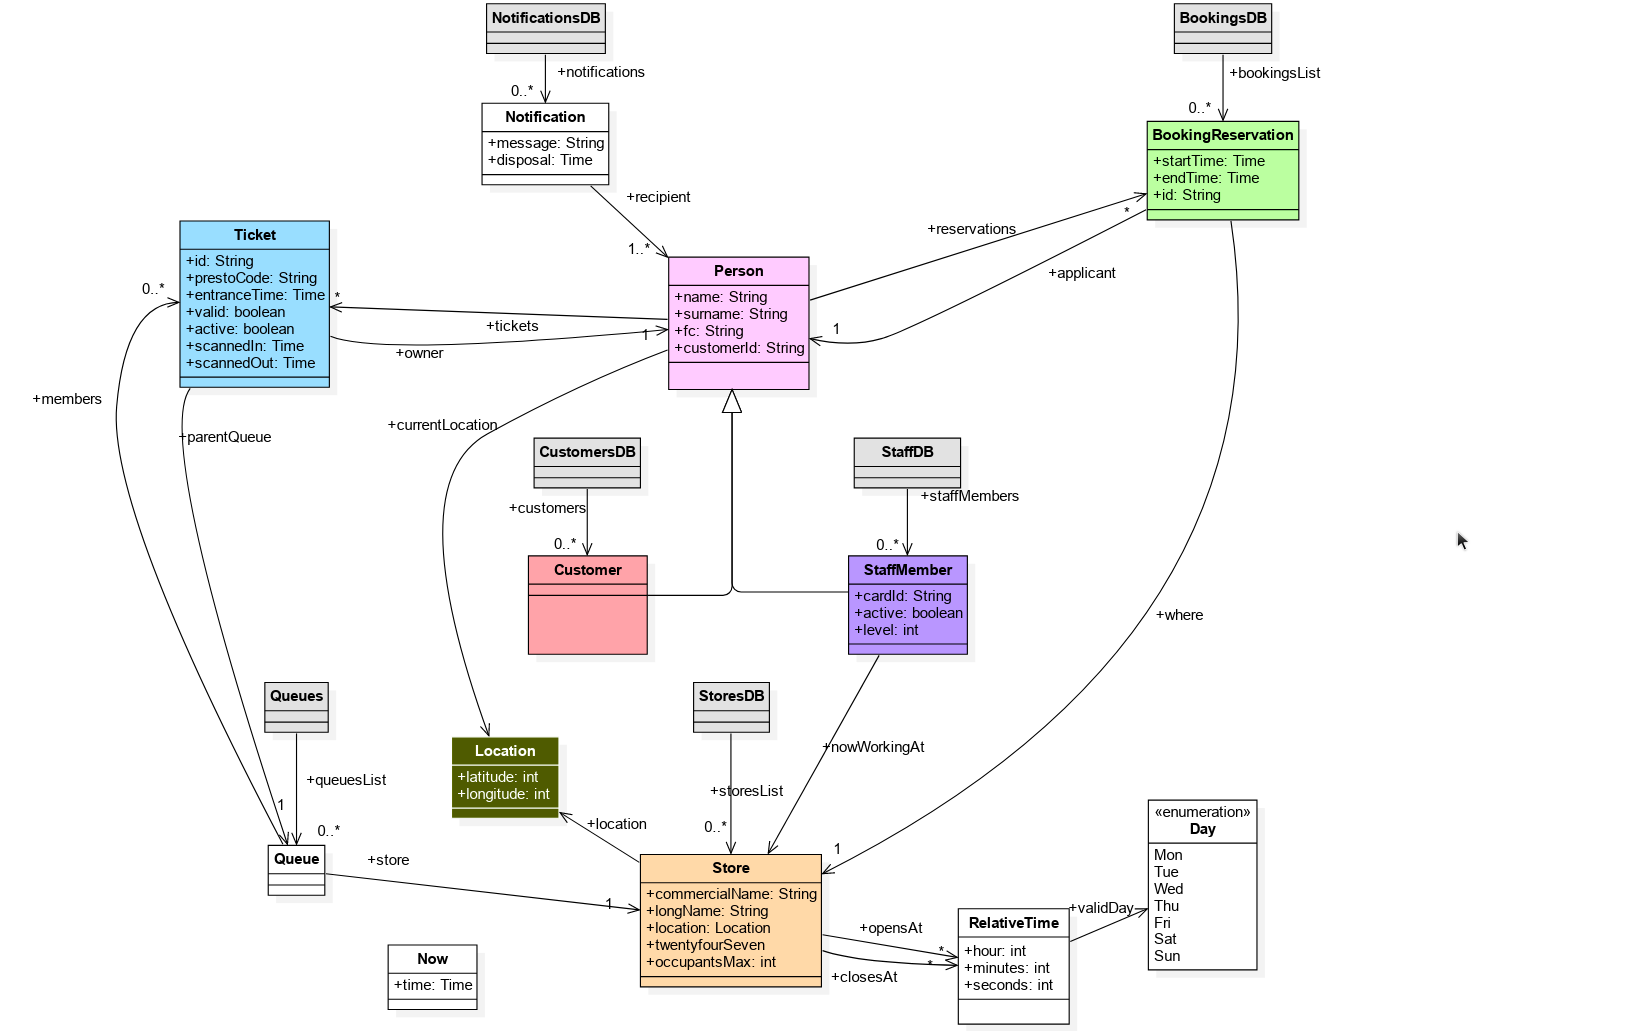
\includegraphics[width=\linewidth]{../Diagrams/main_class_diagram.png}
	\caption{UML: class diagram.}
	\label{fig:UML}
\end{figure}
CLup is an application aiming to decrease the hazard of contracting COVID-19 (or other contagious diseases) when going shopping to a supermarket. The components are two: the main one targets customers of supermarkets while the second one is available for store managers.
Regarding the first component, customers will be required to register to the service the first time they use it by inserting their full name, email address, ID card, phone number and a password. The customer will also be requested to specify his physical address, or to enable the GPS, in order to allow CLup to find stores nearby; this last information can be changed anytime the user needs. If the customer is not willing to register or share his address, the service will not be available.
Once the setup is done the customer is now able to access the homepage of the application, here he can tap on the button “Virtually queue” that allows him to see a list of stores inside a specified range from his location: for every store it is also specified the distance in kilometers from the user position, the number of people inside the store and its maximum occupancy, if the store is full it is instead displayed the number of people in line and the EWT.  It is also possible to visualize stores on a map and, by tapping on one of them, to see the same information displayed in the list. Now, if the user chooses to reserve a spot in the line, the application will open a confirm dialog specifying EWT and the expiration of the ticket. If the user refuses nothing happens, if he accepts instead CLup will process the request, show his ticket and the real time evolution of the line; the ticket is also visible from a home button. The process is shown in Figure ~\ref{fig:VirtuallyQ}.\\
The distance range in which CLup will look for supermarkets is specified by the user through the filter button in the homepage, this button will in fact open the filter screen in which, among other parameters, a sliding bar controls the distance and a dropdown list allows the user to filter the chains of supermarkets.\\

\begin{figure}
	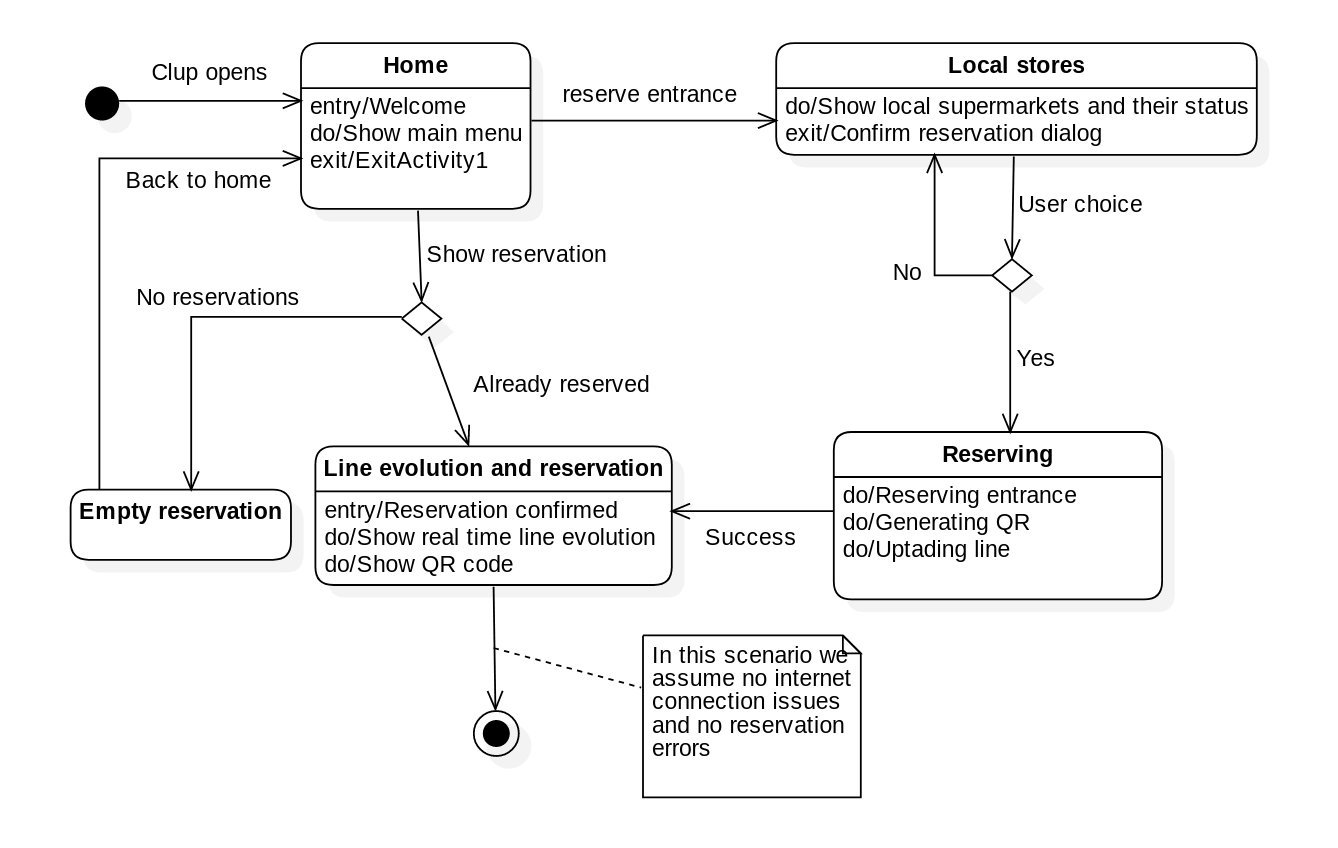
\includegraphics[width=\linewidth]{../Diagrams/VirtuallyQueue.png}
	\caption{Statechart diagram: Virtually queue.}
	\label{fig:VirtuallyQ}
\end{figure}

Another important feature is the possibility to book an entrance later in the day or in another day. The user can specify from the filters whether he prefers to choose the day or the store first and he can set the time range in which he wants to book. 
There is a dedicated button in the app’s main screen that redirects the user to either the list/map of supermarkets or the calendar, and once the user chooses he will be respectively shown the calendar or the list/map, this time with colours to indicate the average crowdedness of stores/days given the set time range.
When the user chooses the day and supermarket combination, a timetable spanning the chosen time range is shown, divided in 15 minutes time slots each one having again a colour to indicate the crowdedness. The user will be able to check his reservation on the home page and near the entrance time he will be provided an actual ticket. The process is shown in Figure ~\ref{fig:BookEntr}.\\

\begin{figure}
	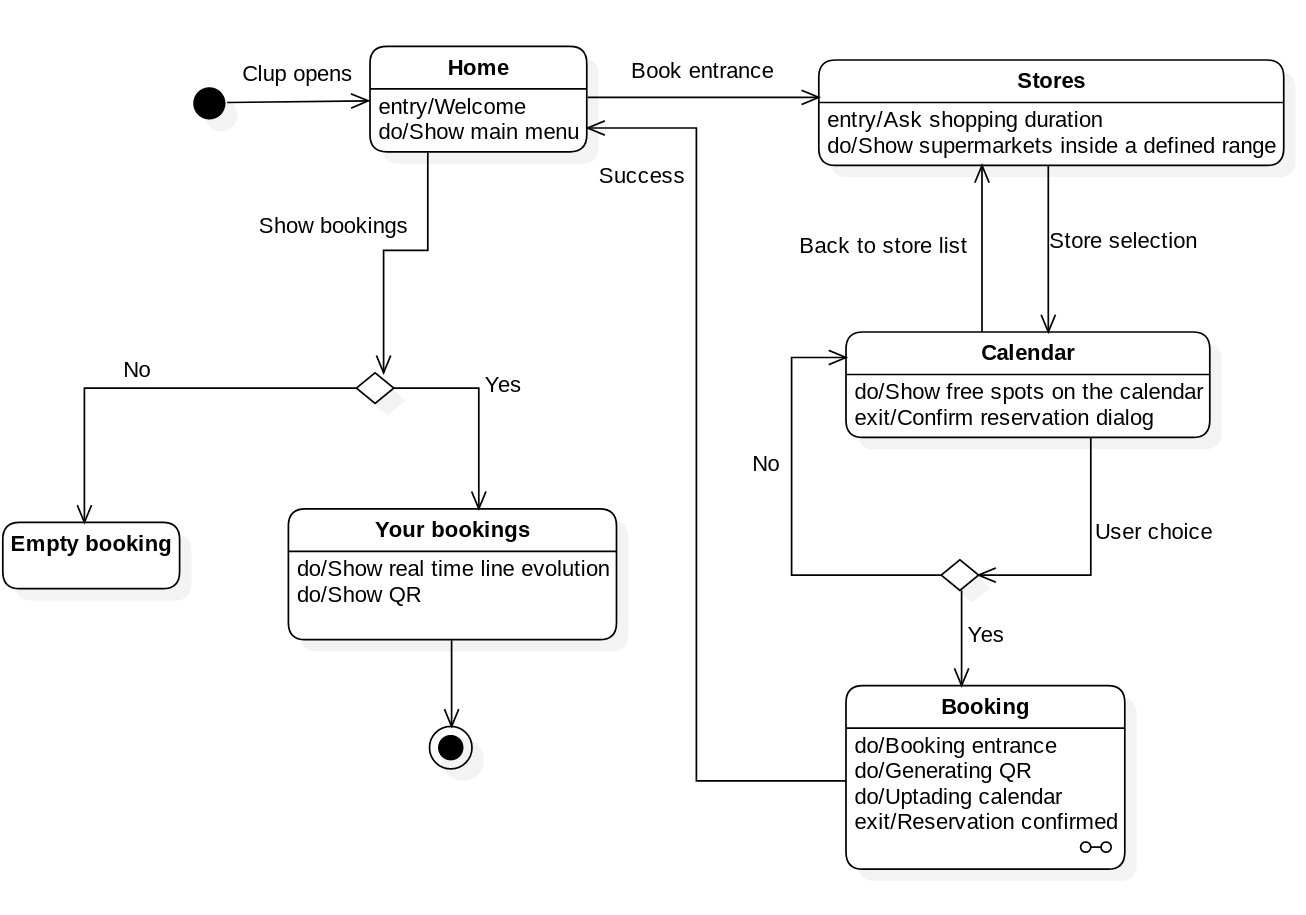
\includegraphics[width=\linewidth]{../Diagrams/BookEntrance.png}
	\caption{Statechart diagram: Book Entrance.}
	\label{fig:BookEntr}
\end{figure} 

The access at the supermarket is restricted by turnstiles with QR code readers, a staff member is expected to verify that nobody waits his turn in front of the entrance, jumps the turnstile or does anything irresponsible.\\
Customers which, for any reason, don’t use the app will still be able to queue in CLup supermarkets by obtaining a printed ticket from a physical totem located near such stores; the functioning of the application will be similar to the “Quick ticket” app function with the difference that the user can only obtain a ticket for the totem’s store. \\
The tickets consist of a QR code and an easy to remember alphanumeric code alternative to enter the store. There will also be monitors that show the numbers allowed to enter and, eventually, delays.\\
The second component of CLup targets store managers: when the store decides to join the CLup network, the credentials to access the web app will be given. In this way the application will have a dedicated section to display flux data of the store selected (Che dati nello specifico? Interazione con i dati???Visualizzazione dati e possibilità di sospendere il servizio)

\subsubsection{\sffamily Scenarios}
\paragraph{Scenario 1}

Single user of the CLup platform, Bob, decides it's time to go shopping.
Bob lives in Milan and this means he's currently in reach of \textbf{5 different supermarkets} belonging to the CLup network. \newline
Bob then opens the app, checks the status of the current queue and notices the nearest supermarket has free room, 13 entrances left out of 55 total. It's fine for Bob, he starts walking towards it.

As soon as he approaches the supermarket (Bob's on foot), he checks the app and start the \textbf{check-in procedure}. It's not rush hours and 8 entrance are still left, so everything goes ok and Bob gets a \textbf{QR ticket}. He approaches the entrance, has his code \textbf{scanned by an automatic turnstile} and gets inside the supermarket.\newline
In 36' time, Bob completes his shopping. He proceeds towards the exit, where another turnstile \textbf{scans his QR code once again to confirm exit}. He's now free to get home.

\paragraph{Scenario 2}

Clara, mother of three children, now needs to go shopping. She's just downloaded CLup and has not figured out how to use it yet.

Clara decides to have a try right now, on the fly, and opens the app to check for local available supermarkets. 
\newline Unfortunately it's now \textbf{rush hours}, hence 2 of the 3 local supermarket show no currently available entrances and an \textbf{e.w.t. of 35 minutes}. Young mother decides to click on ``Reserve entrance'' and notices she has \textbf{15 minutes left to enter the store}. This is done in order to minimize false reservations impact on the service's availability.

Clara has to travel a 4 Km distance in her home town which seems reasonable, but since it's rush hours, \textbf{actually requires 25 minutes of time} to be travelled by car: her QR code has expired.\newline
Fortunately, she checks CLup and can now see new free accesses in the other 2 CLup powered supermarkets, the nearest of which is only a kilometer away. She then reserves an access, reaches the supermarket in 10' time and is now free to do her shopping.

\paragraph{Scenario 3}
James is a young unemployed man, living in the west, outer side of Rome. His \textbf{not particularly wealthy} condition does not overcome his strong medical conceptions, so that he's \textbf{particularly committed in avoiding queues} and other possible ways of contracting Covid-19 in general.

His fridge is starting to starve, so James - who still relies on a well aged Nokia 3310 for its calls and messaging - decides to go shopping. Despite being \guillemotleft less tech-ready\guillemotright \space than average, James has nonetheless heard about a new app (a new way) of shopping and decides to give CLup powered supermarkets a try. Those with the lit CLup mark outside.
\newline The nearest of the two eligible supermarkets in James' reach is 900m away and he's on foot. \textbf{Owning no smartphone}, James considers a reasonably not crowded time to go, 3 p.m., and walks towards the store. 

Unfortunately James' guessing is wrong and the supermarket is \textbf{full}: a \textbf{big screen notifies no entrance is allowed for now}, and everybody has to stay clear of the entrance. He knows no alternative store as he owns no smartphone, but notices the big screen at the entrance has advices for him: next to the entrance, there's a \textbf{self service area} - enclosed by barriers and accessed by automated turnstiles - where James can have a ticket printed. \textbf{Only one person at a time} is allowed in, so that James and anybody else has nothing to worry about.
\newline Right after printing its QR, James can notice the big screen now shows information about it, giving him (better, its ticket number, which reads AX625RQ) advice to \textbf{come back in 20 minutes} for entrance. He then goes for a walk.

25 minutes later James approaches the supermarket and a \textbf{\textcolor{green} {green line}} on the big screen says the owner of ticket AX625RQ is allowed to enter the store for another 10 minutes. 
\newline James happily heads towards the entrance door, has its paper ticket scanned at the turnstiles and enjoys its queue-less shopping.

\paragraph{Scenario 4}
Sara is another young, unemployed woman who lives in an outer borough of Naples. She does own a smartphone, even though it's a bit \textbf{old and sometimes sluggish} in the use. She uses it primarily for texting even though CLup is installed and seems to work.

It's 10 am and Sara needs to go shopping, so opens up CLup and reserves an entrance to the nearest store. She reaches the entrance, looks for her QR code and notices \textbf{her smartphone is suddenly misbehaving}, randomly rebooting and not letting her accomplish the task. \newline
She could have memorized her \textit{presto code} but she actually did not, and asking for a manual check-in is not an option since human interactions have to be avoided - the staff would not let her in.

Sara feels annoyed, and decides she has no time to spend waiting for her smartphone to get back to normal, so she will try and access \textbf{like an offline customer}. The store is almost empty but some other offline customers are to get their tickets. \newline
She looks at the big screen over the entrance, someone is currently occupying the self area but that particular store has room for 5 consecutive offline customers, so she enters the fenced area, stopping at \guillemotleft one turnstile distance\guillemotright \space from the guy currently occupying the self area. In 2 minutes approximately, Sara is able to reach the self machine, have a new ticket printed and get back out.

The big screen announces both the offline tickets are allowed in (there's few persons inside), hence Sara heads towards the turnstiles and gets inside the supermarket, on her way to buying her next smartphone.


\paragraph{Scenario 5}

Michael's family lives outside Messina, in a nice cottage by the sea. Panorama is beautiful, going shopping though requires some effort. \newline
Either Michael or his wife, Laura, have to take the car and travel 25 kilometers of state road to the city. This typically requires up to 1 hour in rush hours, and 35 minutes on average.

This is the type of situation in which the possibility of \textbf{booking} an entrance comes in handy. It's 11.30 a.m.: Laura opens CLup and books an entrance at 5 p.m., providing an estimated shopping time of 1 hour. \newline
CLup's \textbf{alternative stores functionality} also plays a fundamental role for Laura and her family, as they often head towards Ganzirri - another city on Sicily's east coast, opposite direction than Messina - to do their shopping. There are other shopping districts down there, typically less crowded and easier to reach. Today's best alternative happens to be a supermarket in Messina city though.

At 4.10 pm, Laura gets in the car and heads towards the booked store. She arrives at 5.05 p.m, has her QR booking code scanned and gets in. \newline
However, children are usually hungry and Laura's three kids make no exception to this. She hurries getting the job done quickly, but she inevitably ends up \textbf{exceeding the 1 hour slot she had booked.} \newline
Right now the store is full, and this apparently concerning problem leads CLup system to \textbf{alert with reasonable notice one user}, whose entrance would have been right after Laura's exit, that he will have to wait an additional 15 minutes before entering the store. \newline
In the end, Laura manages to get outside the supermarket 65 minutes after she got in. 


Had she required more than that, at 71st minute CLup would have warned the aforementioned user to add another 10 minutes delay to his entrance, and so forth. So that everybody stays safe and \textbf{no overcrowding} takes place.\newline
Straightforwardly enough, Laura's \textbf{delay inevitably becomes root of possible discomfort.} Nonetheless, CLup engine makes note of Laura's behaviour and adds her last shopping time to her personal data: this is going to be taken into account the next time she books a visit, and over time the system will become able to \textbf{forecast her actual shopping time}, thus reducing consequent discomforts.\newline
It is worth noting that this really unfortunate situation generates a problem since Laura's delay occurs specifically when the store is full, condition without which the problem would not have been so concerning.\newline
Also, comparing CLup management of the situation with standard management indicates a \underline{fairly good improvement}: without CLup, the next customer could not have booked its visit (much less, being warned about delays), but instead he would simply have reached the store at 7 p.m and crowded to wait an indeterminate amount of time outside the store.

\paragraph{Scenario 6}
Valerio is a tech oriented grandfather, whose grandson is committed about technology and pushes him towards the use of electronic devices.\newline
Everything tends to go well, except sometimes Valerio \textit{mis-taps} something on its smartphone. Today Valerio is trying to get used to the new shopping app his grandson has provided him with, and accidentally makes a booking for late afternoon, at 6 o'clock, at a superstore near his house.\newline
Valerio seems not to notice his mistake, and simply closes the app. Hence the booking remains valid.

We again find ourselves in the very unfortunate situation in which, at 6 o'clock the superstore is full and Valerio's booking means one less entrance for someone who needed it. This actually represents a problem for the very next 15 minutes after 6 p.m., since at 6.16 the booking is automatically cancelled and the next user in current queue is notified he can proceed. 

Also, system makes note of Valerio's mistake and reports it to the superstore's Staff. They will be presented a comprehensive report, reading which they will be able to decide whether to contact Valerio for explanations or simply ignore the incident, taking into account factors only humans can evaluate (like Valerio's age).\newline

However, CLup's reservation procedure includes an explicit confirmation dialogue, which is aimed at reducing this type of inconvenience.

\paragraph{Scenario 7}

Let's now talk about Alex. He's a young man, living with some sort of anxiety: he's always worried of being late, loosing his seat, and so on.
Today's day is going to be full of engagements and despite being roughly 7 o'clock a.m, Alex is now making a booking for a shopping during the evening. \newline
Alex opens up CLup, clicks on the booking section and he's immediately presented with a list of 10 supermarkets available in Norcia, where he lives. Alex \textit{chooses not to choose}: he books a slot at 7 p.m. at each one of the 10 supermarkets.

Now, this is a perfectly common situation, potentially induced by other factors - many of which being far less innocent than Alex's. \newline
However, CLup's booking \textbf{system prevents booking more than two entrances on the same day}, hence preventing Alex's behaviour. He is in fact given negative response after the second booking, with a kind informative message explaining the situation.

The reasons behind this are straightforward. CLup aims at \textbf{improving, safening and optimizing the shopping experience} in general for the end user. This of course translates into the possibility of \textbf{shopping planning}, but has to \textbf{prevent prevarication} of some users over others as well. \newline
Alex's behaviour, without this kind of policies, would inevitably reduce the number of persons allowed to go shopping at the same time, failing aforementioned purposes and possibly worsening the user experience w.r.t. the current situation.

\paragraph{Scenario 8}

Middle-aged woman Debora also happens to be incline to \guillemotleft compulsive booking\guillemotright, but in a slightly different manner than Alex. \newline
She is used to book services she will not have time to take advantage of in the end, and this also applies to CLup shopping booking. In the last 7 days, she booked a staggering total of 10 different slots, actually never going to the supermarket afterwards.

Again, this kind of situation can be avoided. CLup integrates a customizable policy about \textbf{fake booking prevention} that each store can configure according to their likes. \newline
Between a minimum of 3 and a maximum of 10 fake bookings will result in CLup \textbf{shutting off user's ability to make bookings}, leaving only the ``line up'' functionality available for use. The booking feature may then be restored after manual intervention or a preset amount of time. \newline
\textbf{Note how this is not going to prevent anyone from shopping} - since lining up is always allowed, just like normal - thus guaranteeing goals \texttt{G7}, \texttt{G9} and \texttt{G10}; at the same time though, it helps the booking feature works at its best by reducing disruptions, possibly increasing the overall stores' throughput.

\subsection{Product Functions}
CLup has NNNN main functionalities, each one of them is essential to reach the goals of the application.\\

\subsubsection{Virtually queue in stores}
This is the core of CLup, this function allows the user to virtually queue with a ticket to enter, as soon as possible, the supermarket he chooses. To do this the user needs to set his starting location, his preferred store chains and the distance range in which the application should look for stores, then CLup will present the stores located inside that range in form of a sorted list or a map with supermarkets highlighted. The list specifies for each store the distance from the starting location, the EWT to enter based on the size of the store and the number of people who already have a ticket for it, the number of people who are already inside and the maximum occupancy. The alternatives sorting system will be discussed later. The information displayed in the list is also visible from the map if the user selects a supermarket. When the user selects a store the application will show him the current EWT to enter and remind him that he has 15 minutes after his turn has come before the ticket definitely expires. Finally it will ask him if he is sure to reserve the entrance. This confirmation dialog is mainly useful to make sure that the user is aware of the timings and he can organize his commitments to go shopping in time. On the other hand, having a confirmation dialog is useful to prevent unintentional reservations by distracted or non-techy users. After the reservation is done, the user can follow the evolution of the line from the application which will give him real time information: the numbers of the tickets that are supposed to enter, the number of people ahead of the user and the estimated wait time. At this point the user should have enough information to arrive at the supermarket neither too early nor too late: in the first case he must wait in the car or away from the store, in the second one his ticket could expire and he would have to get a new one and wait again for his turn. When the time comes, CLup notifies the user that he should enter within 15 minutes. At the entrance the customer scans his QR code, or inserts the code of his ticket, and the turnstile lets him in. Obviously, if the store is not full and it is the turn of many customers to enter CLup allows them to access in any order, if a customer tries to scan the QR at the wrong time, ticket expired or that ticket has not been called yet, the turnstile won’t let him pass. When the shopping is finished the customer scans again his QR code, or inserts the code, notifying the CLup system that there is one more entrance available in that store.
People who do not have the app can still virtually queue by getting a ticket printed from the physical totems near CLup powered stores where there is also a big screen showing the entering ticket numbers. On the printed ticket it is specified the EWT but of course they will miss the possibility to be updated on the queue status because it is forbidden to wait in front of the store, also the totems give tickets only for the store where they are located.
To get more accurate estimations, through the entering and exiting turnstiles, the system stores the shopping time of each user in order to build statistics. 
To avoid abuses of this function, it is not possible to reserve more than one entrance at the same time, the user will be able to reserve another entrance on the same day only after he left the first store. For the same reasons it will be later described that the store managers can prevent users from making new reservations if they let too many tickets expire..


\subsubsection{Book entrance}
This feature allows the user to book a ticket to enter in a specific time slot of a specific day, it is available in the mobile app and targets users who want to schedule their shopping time instead of just going as soon as possible. Just as for the previous function, the user needs a little setup for the starting location and eventually other filters, then he can visualize the matching solutions starting either from a list or a map, or starting from a calendar., Either of the starting views then takes the user to the other one (general calendar -> map/list for that day,  general map/list -> calendar for that store) and after selecting both the store and the day a list of time slots for that day will be shown. Once the user decides the combination of store, day and time he can go on with the booking procedure and book his slot by giving confirmation. The application will process his request and, when the time comes, the application will generate the QR code (and notify the user) one hour in advance, from there the user will have 1:15 hours to enter the store before the ticket expires. If the user arrives early, even if the store is empty, the QR will only be valid for the chosen time. From this point on, the functioning is just as in the previous feature.\\
Also in this case abuses are discouraged: it is not possible to book more than an entrance per day and a ban mechanism is implemented, Clup counts the number of times a user reserves an entrance and then does not go to the store, if this value exceeds a threshold selected by the supermarket the user can not book an entrance to that supermarket until the number of booking absence is reset two weeks after  .

\subsubsection{Suggestions among different stores and times}
This function was actually anticipated in the previous ones and aims at balancing the flux of people between stores and between different hours but, while the previous ones had a dedicated interface button, this one works in background: when the user wants to book or reserve an entrance, if he chooses to visualize stores in list mode, the list is accurately sorted with the purpose of putting in first place the least crowded stores and those with fewer probability of being chosen by other customers based on the statistics. If the user chooses the map visualization each store will have associated a color that indicates its crowdedness. In any case CLup will notify the user if there is a better solution outside of the set filters. 

\subsubsection{Store management} 
This function is only for the store managers, it allows them to:
\begin{itemize}
	\item
	\textbf{view affluence statistics}: the manager can see the status of the supermarket crowdedness, the line to enter, the calendar with all the booked entrances and the throughput. However store managers
	\item
	\textbf{stop new entrances}: temporarily prevent coming users with valid tickets from entering the store
	\item
	\textbf{change current store capacity}: set the maximum capacity of the store at a certain time so that the automatic queuing system can plan the queue accordingly
	\item
	\textbf{inspect misbehaving user automatically generated reports}: The system automatically generates reports from users who miss their reservations or take too long shopping in the supermarket, these are then merged into statistics that allow the managers to use in an informed manner the next feature in this list
	\item 
	\textbf{block or unblock users from accessing CLup for a certain store}: given the reports it is possible to prevent some users from reserving tickets, or also it is possible to let a user reserve again after an eventual clarification with him. It is also possible to set thresholds for which the system automatically blocks or unblocks users
\end{itemize}


\subsection{User Characteristics}
The application targets two different entities: users and store managers.
\begin{itemize}
	\item
	\textbf{Users} are the main concern of CLup, they represent every customer of supermarkets and actually differentiate between registered and offline users, they need to shop and they need to do it safely. They want to shop at stores without waiting outside and by spending as little time as possible using the application or totem, for this reason the application is very simple and intuitive.
	\item
	\textbf{Store managers} are supermarket accountants willing to find safer shopping solutions for their customers and their staff.
\end{itemize}



\subsection{Assumptions, Dependencies and Constraints}
\subsubsection{Domain Assumptions}
Follows a list of assumptions made about the domain CLup focuses on.\newline\newline
\begin{tabular}{l|l}
	D1 & Accesses to the store can be monitored\\
	D2 & Exits from the store can be monitored\\
	D3 & One customer per authorization given is allowed in by the Staff\\
	D4 & Users are reasonably able to manage their time while following the queue evolution\\
    D5 & Users can estimate the time required to arrive to the store\\
    D6 & Users who arrives too early at the supermarket don't wait in front of the entrance\\
    D7 & Customers keep the safe distance\\
    D8 & Malicious users are not enough in number or coordination to prevent Clup to work\\
    D9 & Users insert the right starting location or their GPS works\\
    D10 & Store managers give the right information about supermarkets\\
    D11 & Staff guarantees access control systems operativeness\\
	
\end{tabular}

\paragraph{Scenario 4}
Sara is another young, unemployed woman who lives in an outer borough of Naples. She does own a smartphone, even though it's a bit \textbf{old and sometimes sluggish} in the use. She uses it primarily for texting even though CLup is installed and seems to work.

It's 10 am and Sara needs to go shopping, so opens up CLup and reserves an entrance to the nearest store. She reaches the entrance, looks for her QR code and notices \textbf{her smartphone is suddenly misbehaving}, randomly rebooting and not letting her accomplish the task. \newline
She could have memorized her \textit{presto code} but she actually did not, and asking for a manual check-in is not an option since human interactions have to be avoided - the staff would not let her in.

Sara feels annoyed, and decides she has no time to spend waiting for her smartphone to get back to normal, so she will try and access \textbf{like an offline customer}. The store is almost empty but some other offline customers are to get their tickets. \newline
She looks at the big screen over the entrance, someone is currently occupying the self area but that particular store has room for 5 consecutive offline customers, so she enters the fenced area, stopping at \guillemotleft one turnstile distance\guillemotright \space from the guy currently occupying the self area. In 2 minutes approximately, Sara is able to reach the self machine, have a new ticket printed and get back out.

The big screen announces both the offline tickets are allowed in (there's few persons inside), hence Sara heads towards the turnstiles and gets inside the supermarket, on her way to buying her next smartphone.


\paragraph{Scenario 5}

Michael's family lives outside Messina, in a nice cottage by the sea. Panorama is beautiful, going shopping though requires some effort. \newline
Either Michael or his wife, Laura, have to take the car and travel 25 kilometers of state road to the city. This typically requires up to 1 hour in rush hours, and 35 minutes on average.

This is the type of situation in which the possibility of \textbf{booking} an entrance comes in handy. It's 11.30 a.m.: Laura opens CLup and books an entrance at 5 p.m., providing an estimated shopping time of 1 hour. \newline
CLup's \textbf{alternative stores functionality} also plays a fundamental role for Laura and her family, as they often head towards Ganzirri - another city on Sicily's east coast, opposite direction than Messina - to do their shopping. There are other shopping districts down there, typically less crowded and easier to reach. Today's best alternative happens to be a supermarket in Messina city though.

At 4.10 pm, Laura gets in the car and heads towards the booked store. She arrives at 5.05 p.m, has her QR booking code scanned and gets in. \newline
However, children are usually hungry and Laura's three kids make no exception to this. She hurries getting the job done quickly, but she inevitably ends up \textbf{exceeding the 1 hour slot she had booked.} \newline
Right now the store is full, and this apparently concerning problem leads CLup system to \textbf{alert with reasonable notice one user}, whose entrance would have been right after Laura's exit, that he will have to wait an additional 15 minutes before entering the store. \newline
In the end, Laura manages to get outside the supermarket 65 minutes after she got in. 


Had she required more than that, at 71st minute CLup would have warned the aforementioned user to add another 10 minutes delay to his entrance, and so forth. So that everybody stays safe and \textbf{no overcrowding} takes place.\newline
Straightforwardly enough, Laura's \textbf{delay inevitably becomes root of possible discomfort.} Nonetheless, CLup engine makes note of Laura's behaviour and adds her last shopping time to her personal data: this is going to be taken into account the next time she books a visit, and over time the system will become able to \textbf{forecast her actual shopping time}, thus reducing consequent discomforts.\newline
It is worth noting that this really unfortunate situation generates a problem since Laura's delay occurs specifically when the store is full, condition without which the problem would not have been so concerning.\newline
Also, comparing CLup management of the situation with standard management indicates a \underline{fairly good improvement}: without CLup, the next customer could not have booked its visit (much less, being warned about delays), but instead he would simply have reached the store at 7 p.m and crowded to wait an indeterminate amount of time outside the store.

\paragraph{Scenario 6}
Valerio is a tech oriented grandfather, whose grandson is committed about technology and pushes him towards the use of electronic devices.\newline
Everything tends to go well, except sometimes Valerio \textit{mis-taps} something on its smartphone. Today Valerio is trying to get used to the new shopping app his grandson has provided him with, and accidentally makes a booking for late afternoon, at 6 o'clock, at a superstore near his house.\newline
Valerio seems not to notice his mistake, and simply closes the app. Hence the booking remains valid.

We again find ourselves in the very unfortunate situation in which, at 6 o'clock the superstore is full and Valerio's booking means one less entrance for someone who needed it. This actually represents a problem for the very next 15 minutes after 6 p.m., since at 6.16 the booking is automatically cancelled and the next user in current queue is notified he can proceed. 

Also, system makes note of Valerio's mistake and reports it to the superstore's Staff. They will be presented a comprehensive report, reading which they will be able to decide whether to contact Valerio for explanations or simply ignore the incident, taking into account factors only humans can evaluate (like Valerio's age).\newline

However, CLup's reservation procedure includes an explicit confirmation dialogue, which is aimed at reducing this type of inconvenience.

\paragraph{Scenario 7}

Let's now talk about Alex. He's a young man, living with some sort of anxiety: he's always worried of being late, loosing his seat, and so on.
Today's day is going to be full of engagements and despite being roughly 7 o'clock a.m, Alex is now making a booking for a shopping during the evening. \newline
Alex opens up CLup, clicks on the booking section and he's immediately presented with a list of 10 supermarkets available in Norcia, where he lives. Alex \textit{chooses not to choose}: he books a slot at 7 p.m. at each one of the 10 supermarkets.

Now, this is a perfectly common situation, potentially induced by other factors - many of which being far less innocent than Alex's. \newline
However, CLup's booking \textbf{system prevents booking more than two entrances on the same day}, hence preventing Alex's behaviour. He is in fact given negative response after the second booking, with a kind informative message explaining the situation.

The reasons behind this are straightforward. CLup aims at \textbf{improving, safening and optimizing the shopping experience} in general for the end user. This of course translates into the possibility of \textbf{shopping planning}, but has to \textbf{prevent prevarication} of some users over others as well. \newline
Alex's behaviour, without this kind of policies, would inevitably reduce the number of persons allowed to go shopping at the same time, failing aforementioned purposes and possibly worsening the user experience w.r.t. the current situation.

\paragraph{Scenario 8}

Middle-aged woman Debora also happens to be incline to \guillemotleft compulsive booking\guillemotright, but in a slightly different manner than Alex. \newline
She is used to book services she will not have time to take advantage of in the end, and this also applies to CLup shopping booking. In the last 7 days, she booked a staggering total of 10 different slots, actually never going to the supermarket afterwards.

Again, this kind of situation can be avoided. CLup integrates a customizable policy about \textbf{fake booking prevention} that each store can configure according to their likes. \newline
Between a minimum of 3 and a maximum of 10 fake bookings will result in CLup \textbf{shutting off user's ability to make bookings}, leaving only the ``line up'' functionality available for use. The booking feature may then be restored after manual intervention or a preset amount of time. \newline
\textbf{Note how this is not going to prevent anyone from shopping} - since lining up is always allowed, just like normal - thus guaranteeing goals \texttt{G7}, \texttt{G9} and \texttt{G10}; at the same time though, it helps the booking feature works at its best by reducing disruptions, possibly increasing the overall stores' throughput.

\subsection{Product Functions}
CLup has NNNN main functionalities, each one of them is essential to reach the goals of the application.\\

\subsubsection{Virtually queue in stores}
This is the core of CLup, this function allows the user to virtually queue with a ticket to enter, as soon as possible, the supermarket he chooses. To do this the user needs to set his starting location, his preferred store chains and the distance range in which the application should look for stores, then CLup will present the stores located inside that range in form of a sorted list or a map with supermarkets highlighted. The list specifies for each store the distance from the starting location, the EWT to enter based on the size of the store and the number of people who already have a ticket for it, the number of people who are already inside and the maximum occupancy. The alternatives sorting system will be discussed later. The information displayed in the list is also visible from the map if the user selects a supermarket. When the user selects a store the application will show him the current EWT to enter and remind him that he has 15 minutes after his turn has come before the ticket definitely expires. Finally it will ask him if he is sure to reserve the entrance. This confirmation dialog is mainly useful to make sure that the user is aware of the timings and he can organize his commitments to go shopping in time. On the other hand, having a confirmation dialog is useful to prevent unintentional reservations by distracted or non-techy users. After the reservation is done, the user can follow the evolution of the line from the application which will give him real time information: the numbers of the tickets that are supposed to enter, the number of people ahead of the user and the estimated wait time. At this point the user should have enough information to arrive at the supermarket neither too early nor too late: in the first case he must wait in the car or away from the store, in the second one his ticket could expire and he would have to get a new one and wait again for his turn. When the time comes, CLup notifies the user that he should enter within 15 minutes. At the entrance the customer scans his QR code, or inserts the code of his ticket, and the turnstile lets him in. Obviously, if the store is not full and it is the turn of many customers to enter CLup allows them to access in any order, if a customer tries to scan the QR at the wrong time, ticket expired or that ticket has not been called yet, the turnstile won’t let him pass. When the shopping is finished the customer scans again his QR code, or inserts the code, notifying the CLup system that there is one more entrance available in that store.
People who do not have the app can still virtually queue by getting a ticket printed from the physical totems near CLup powered stores where there is also a big screen showing the entering ticket numbers. On the printed ticket it is specified the EWT but of course they will miss the possibility to be updated on the queue status because it is forbidden to wait in front of the store, also the totems give tickets only for the store where they are located.
To get more accurate estimations, through the entering and exiting turnstiles, the system stores the shopping time of each user in order to build statistics. 
To avoid abuses of this function, it is not possible to reserve more than one entrance at the same time, the user will be able to reserve another entrance on the same day only after he left the first store. For the same reasons it will be later described that the store managers can prevent users from making new reservations if they let too many tickets expire..


\subsubsection{Book entrance}
This feature allows the user to book a ticket to enter in a specific time slot of a specific day, it is available in the mobile app and targets users who want to schedule their shopping time instead of just going as soon as possible. Just as for the previous function, the user needs a little setup for the starting location and eventually other filters, then he can visualize the matching solutions starting either from a list or a map, or starting from a calendar., Either of the starting views then takes the user to the other one (general calendar -> map/list for that day,  general map/list -> calendar for that store) and after selecting both the store and the day a list of time slots for that day will be shown. Once the user decides the combination of store, day and time he can go on with the booking procedure and book his slot by giving confirmation. The application will process his request and, when the time comes, the application will generate the QR code (and notify the user) one hour in advance, from there the user will have 1:15 hours to enter the store before the ticket expires. If the user arrives early, even if the store is empty, the QR will only be valid for the chosen time. From this point on, the functioning is just as in the previous feature.\\
Also in this case abuses are discouraged: it is not possible to book more than an entrance per day and a ban mechanism is implemented, Clup counts the number of times a user reserves an entrance and then does not go to the store, if this value exceeds a threshold selected by the supermarket the user can not book an entrance to that supermarket until the number of booking absence is reset two weeks after  .

\subsubsection{Suggestions among different stores and times}
This function was actually anticipated in the previous ones and aims at balancing the flux of people between stores and between different hours but, while the previous ones had a dedicated interface button, this one works in background: when the user wants to book or reserve an entrance, if he chooses to visualize stores in list mode, the list is accurately sorted with the purpose of putting in first place the least crowded stores and those with fewer probability of being chosen by other customers based on the statistics. If the user chooses the map visualization each store will have associated a color that indicates its crowdedness. In any case CLup will notify the user if there is a better solution outside of the set filters. 

\subsubsection{Store management} 
This function is only for the store managers, it allows them to:
\begin{itemize}
	\item
	\textbf{view affluence statistics}: the manager can see the status of the supermarket crowdedness, the line to enter, the calendar with all the booked entrances and the throughput. However store managers
	\item
	\textbf{stop new entrances}: temporarily prevent coming users with valid tickets from entering the store
	\item
	\textbf{change current store capacity}: set the maximum capacity of the store at a certain time so that the automatic queuing system can plan the queue accordingly
	\item
	\textbf{inspect misbehaving user automatically generated reports}: The system automatically generates reports from users who miss their reservations or take too long shopping in the supermarket, these are then merged into statistics that allow the managers to use in an informed manner the next feature in this list
	\item 
	\textbf{block or unblock users from accessing CLup for a certain store}: given the reports it is possible to prevent some users from reserving tickets, or also it is possible to let a user reserve again after an eventual clarification with him. It is also possible to set thresholds for which the system automatically blocks or unblocks users
\end{itemize}


\subsection{User Characteristics}
The application targets two different entities: users and store managers.
\begin{itemize}
	\item
	\textbf{Users} are the main concern of CLup, they represent every customer of supermarkets and actually differentiate between registered and offline users, they need to shop and they need to do it safely. They want to shop at stores without waiting outside and by spending as little time as possible using the application or totem, for this reason the application is very simple and intuitive.
	\item
	\textbf{Store managers} are supermarket accountants willing to find safer shopping solutions for their customers and their staff.
\end{itemize}



\subsection{Assumptions, Dependencies and Constraints}
\subsubsection{Domain Assumptions}
Follows a list of assumptions made about the domain CLup focuses on.\newline\newline
\begin{tabular}{l|l}
	D1 & Accesses to the store can be monitored\\
	D2 & Exits from the store can be monitored\\
	D3 & One customer per authorization given is allowed in by the Staff\\
	D4 & Users are reasonably able to manage their time while following the queue evolution\\
    D5 & Users can estimate the time required to arrive to the store\\
    D6 & Users who arrives too early at the supermarket don't wait in front of the entrance\\
    D7 & Customers keep the safe distance\\
    D8 & Malicious users are not enough in number or coordination to prevent Clup to work\\
    D9 & Users insert the right starting location or their GPS works\\
    D10 & Store managers give the right information about supermarkets\\
    D11 & Staff guarantees access control systems operativeness\\
	
\end{tabular}
